\documentclass[12pt, a4paper, oneside]{article}
\usepackage{amsmath, amsthm, amssymb, graphicx}
\usepackage[bookmarks=true, colorlinks, citecolor=blue, linkcolor=black]{hyperref}
\usepackage[margin = 25mm]{geometry}
\usepackage{setspace}
\usepackage{listings}
\usepackage{ctex}
\usepackage{float}
\usepackage{fancyhdr}
\title{Title}
\date{\today}
\author{Alphabetium}
\begin{document}
\begin{spacing}{2.0}
\tableofcontents
\maketitle

\section{激光的特点怎样从本质上来解释?}
激光的本质特点可以通过以下几个方面来解释:\\

1.高度相干性:激光的光波具有高度的相干性,这是因为激光中的光子具有几乎相同的频率、相位和方向。相干性可以使激光在空间中表现出干涉和衍射等波动现象。\\

2.高能量密度:激光束的能量密度非常高,这是由于激光具有高度的单色性和方向性,可以将光束聚焦成非常小的斑点,使得在该点上的能量密度非常高。\\

3.窄的频谱线宽:激光的光波频率非常稳定,因此它的频谱线宽非常窄。这使得激光在一些应用领域中能够提供非常高的精度和分辨率。\\

4.窄的方向性:激光的光波具有非常窄的方向性,可以通过透镜或光学器件进行聚焦和控制。这种方向性使得激光在材料加工、光通信和生物医学等领域中具有广泛的应用。
\\
5.短的脉冲宽度:某些类型的激光能够产生非常短的光脉冲,其宽度可在飞秒或皮秒级别内。这种短脉冲的激光在材料加工、光谱学和医学成像等应用中具有独特的优势。
\\
总的来说,激光的本质特点是高度相干性、高能量密度、窄的频谱线宽、窄的方向性和短的脉冲宽度,这些特点使激光在许多应用领域中具有独特的优势和广泛的应用前景。

\section{为什么非稳定腔能产生高功率?}
非稳定腔指的是激光器腔内的谐振条件不是完全稳定的情况,这种腔形态下产生的激光具有较高的峰值功率和短脉冲宽度。下面是一些可能导致非稳定腔产生高功率的原因:\\

1.模式竞争:当激光腔内有多个横模式时,这些模式之间会相互竞争,导致激光产生瞬态过程。这种模式竞争可能导致激光器在短时间内产生较高的峰值功率。
\\
2.自脉冲现象:自脉冲现象指的是激光腔内的激光发生不稳定振荡,产生自发脉冲。这种现象通常是由于激光腔内的反射率、增益介质等参数的变化引起的,自脉冲可以产生非常高的峰值功率。
\\
3.谐振腔失稳:当激光器腔内的谐振条件失稳时,会产生瞬态振荡和高功率激光脉冲。例如,当激光器中的反射镜之间的距离不是完全恒定时,会导致腔内的谐振条件失稳。
\\
总的来说,非稳定腔产生高功率的原因可能是模式竞争、自脉冲现象和谐振腔失稳等。这些现象导致激光器在短时间内产生高峰值功率的脉冲,从而可以应用于一些需要高能量密度和短脉冲宽度的应用中,如材料加工、激光成像和医学治疗等。





\section{形成激光的条件(必要、充分)? }
要形成激光,必须满足下列两个条件:
\\
1.反转粒子分布:反转粒子分布是指激光工作介质中存在一定的粒子数处于高能级状态,而低能级状态的粒子数较少。这种粒子数分布称为反转粒子分布。为了实现反转粒子分布,需要给激光工作介质提供足够的能量,将其激发到高能级状态,然后通过非自发辐射(如吸收和受激辐射等)使其回到低能级状态。只有存在反转粒子分布,才能产生激光放射。
\\
2.谐振腔:谐振腔是指激光器内的两个反射镜,它们之间的距离为光波长的整数倍。这种谐振腔可以将产生的光束反复反射回去,使得激光光束在腔内不断放大和自放大。在谐振腔内,激光光束反复通过激光工作介质,使得介质中的反转粒子数不断增加,并最终达到产生激光放射的阈值。
\\
因此,形成激光的条件是必须具有反转粒子分布和谐振腔。反转粒子分布是产生激光放射的物理基础,而谐振腔则是激光放大和自放大的场所。

\section{可以用哪几种方法表示阈值条件? }
阈值条件是指在激光工作介质中需要满足一定的条件才能产生激光放射。通常可以用下面三种方法来表示阈值条件:
\\
1.折射率法:该方法通过计算激光在激光工作介质中的传输损失和谐振腔的增益来得到阈值条件。当激光损失和增益相等时,就可以得到阈值条件。
\\
2.光谱法:该方法通过测量激光工作介质在某一波长下的吸收光谱和受激辐射光谱,计算其增益系数和损失系数,然后求得阈值条件。
\\
3.激光脉冲法:该方法是在激光工作介质中输入一个脉冲激励光,在腔内产生激光脉冲,然后通过改变脉冲激励光的强度来寻找激光脉冲的阈值条件。在阈值条件下,输出的激光脉冲能量呈指数增长,而不是线性增长。
\\
这些方法都是从不同的角度来描述阈值条件,可以根据实验需要和条件选择不同的方法。


\section{从谐振腔分析激光单色性好原因}

激光器的谐振腔是由两个反射镜组成的光学腔,其中一个反射镜是部分透明的,用于输出激光。谐振腔对于激光的单色性有很大的影响,具体来说,谐振腔对于激光单色性好的原因有以下几个方面:
\\
1.频率选择性:谐振腔对于不同频率的光具有不同的反射率和传输率,只有符合共振条件的光才能在腔内传输和反射,其它频率的光则会被过滤掉,从而实现了频率选择性,这是激光器单色性好的重要原因之一。
\\
2.调制深度:由于激光谐振腔内的光场强度很高,使得谐振腔中的介质在光场的作用下发生调制,例如由于Kerr效应等非线性效应而导致折射率的改变,从而影响谐振腔内的模式结构和共振条件,进一步提高了激光的单色性。
\\
3.相位稳定性:谐振腔内的光在传播过程中受到多次反射和传输,这些反射和传输会改变光的相位,但是由于谐振腔内的光程是固定的,因此可以使得反射光和传输光的相位保持稳定,进一步提高了激光的单色性。
\\
综上所述,激光器的谐振腔通过频率选择性、调制深度和相位稳定性等多种机制,能够使激光具有很好的单色性。

\section{实现稳定态条件? }
激光器的稳定态条件是指在激光器的工作过程中,能够保持激光输出功率和光谱特性的稳定性。为了实现稳定态条件,需要满足以下几个方面:
\\
1.能量平衡:激光器内部的能量损失必须与激光输出功率的增益相平衡。能量损失主要包括光学元件吸收和散射损耗、光学腔中介质吸收和非线性效应损耗等。
如果能量损失大于增益,激光器将无法产生稳定输出。
\\
2.泵浦功率稳定:激光器的泵浦光源必须稳定,以确保激光器的增益稳定。泵浦光源的波长、功率和空间模式等特性都需要精确控制。
\\
3.温度稳定:激光器内部的介质折射率随温度变化而变化,因此需要控制激光器的工作温度以保持稳定输出。
\\
4.模式控制:激光器内部可能存在多种不同的激光模式,这些模式的输出功率和光谱特性都不同。为了获得稳定的激光输出,需要采用模式控制技术,例
如模式选择器或模式锁定器等。
\\
综上所述,实现稳定态条件需要精确控制多个因素,包括能量平衡、泵浦功率稳定、温度稳定和模式控制等,以确保激光器的稳定输出。

\section{模竞争}
激光器中可能存在多种激光模式,这些模式的输出功率和光谱特性不同。当这些模式之间存在相互作用时,就会出现模竞争现象。模竞争是指不同激光模式之间的竞争,
导致激光输出的特性不稳定,例如光谱宽度增大、脉冲波形不规则等。

模竞争的主要原因是不同的激光模式具有不同的增益和损耗,而这些因素又受到激光器内部的非线性效应的影响。因此,
不同的激光模式在激光器内部的传输和放大过程中可能出现竞争现象。例如,某些模式具有较高的增益,容易得到放大,因此会占据更多的激光功率;
而其他模式则可能受到较大的损耗,导致输出功率下降。这些模式之间的竞争可能导致激光输出不稳定,严重时甚至会使激光器无法正常工作。

为了避免模竞争现象,可以采用一些模式控制技术,例如模式选择器、模式锁定器等。这些技术可以有效地压制非稳定模式,保持激光输出的稳定性和单色性。

\section{从振荡模式理解空间烧孔效应}
空间烧孔效应(Spatial Hole Burning,简称SHB)是激光器中常见的非线性效应之一,主要是由于激光器中的振荡模式分布不均匀引起的。
在激光器中,激光光波在振荡腔内反复传播,形成了一个复杂的空间场分布。这个场分布由振荡模式的空间分布决定,不同的振荡模式之间相互作用会影响其场分布,
从而导致振荡模式的分布出现变化。

当激光器中某个振荡模式的增益过大时,就会引起空间烧孔效应。这是因为该振荡模式的场强较大,
与其相邻的振荡模式的场强相对较弱,因此该模式的增益会进一步增加。这会导致激光场在该模式处产生局部的光强增益,
从而引起相邻模式的场强下降。这种相互作用会导致模式的分布不均匀,形成空间烧孔。

空间烧孔效应会导致激光器输出功率降低、光谱变宽、波形不稳定等问题。为了避免空间烧孔效应,可以采取一些措施,
如增加激光器的长度、采用多腔设计、使用空间滤波器等。这些方法可以改变振荡模式的分布,从而减少振荡模式之间的相互作用,降低空间烧孔效应的影响。



\section{$\nu$牵引效应}
$\nu$牵引效应(the $\nu$-Trapping effect)是指在激光中介质中,由于介质中的色散特性而导致光的频率被限制在一个窄的带宽范围内,
同时在该带宽范围内,光可以与介质中的电子发生共振作用,这种现象也被称为局域共振或者谐振。

当激光入射介质时,其中的光波与介质中的电子发生相互作用,从而在介质中形成折射率的折射率调制,同时也会在激光中形成一定的相位调制。
这些调制会随着光波在介质中的传播而逐渐累积,从而导致光的频率被限制在一个窄的范围内。

由于这种频率限制的效应,当光在介质中传播时,它将与介质中的电子发生局域共振或者谐振,从而产生一个所谓的$\nu$牵引效应,
即光波会被牵引向与介质中电子的频率相匹配的方向传播。这种效应在一些光学器件中具有实用价值,比如在光纤陀螺仪、光子晶体等器件中都有应用。



\section{模的频率}
在激光中,模式频率是指谐振腔中的场的稳定振荡频率。谐振腔的模式频率可以通过以下公式计算:

$f_{mn}=\frac{c}{2L}\sqrt{m^2+n^2}\qquad(m,n=1,2,3,\cdots)$

其中,$m$和$n$是模式的纵向和横向振动次数,$L$是谐振腔长度,$c$是光速。

例如,在一个具有镜面反射器的二极管激光器中,长边缘沿着x轴,短边缘沿着y轴,当它们产生振荡时,能够产生许多模式。对于$x$和$y$方向上的模式,
模式频率可以分别表示为:

$f_{mnx}=\frac{c}{2L_x}\sqrt{m^2+n^2}\qquad(m,n=1,2,3,\cdots)$

$f_{mny}=\frac{c}{2L_y}\sqrt{m^2+n^2}\qquad(m,n=1,2,3,\cdots)$

在激光器中,通常只有一种或少数几种模式频率处于共振状态,即在腔中建立稳定的场分布。这些频率通常对应于腔长$L$、激光材料的折射率和激光器的工作温度等因素。

\section{连续激光器输出功率与最佳透过率}

对于连续激光器,输出功率与最佳透过率之间存在一个关系,即输出功率随着最佳透过率的增加而增加,但是当最佳透过率达到一定值时,
输出功率将不再增加而保持稳定。这是因为在过高的透过率下,激光材料的吸收损耗会减小,但是反射损耗会增加,从而导致激光器的效率下降。

最佳透过率取决于激光器的工作波长、材料特性、谐振腔的几何形状和其他参数。对于一般的激光器,最佳透过率通常在$30\%-50\%$之间。
在实际应用中,需要对激光器进行实验和测试来确定最佳的透过率,以获得最大的输出功率和最高的效率。
\section{集成光学}
集成光学是一种将光学器件或光学元件集成在单一芯片上的技术。它使用光子晶体材料、半导体材料、光波导、微镜等技术,
将多个光学器件集成在同一芯片上,从而实现高度集成化和紧凑性。

与传统的离散光学器件相比,集成光学器件具有体积小、重量轻、可靠性高、功耗低、调谐灵活、光路稳定等优点。
集成光学技术在通信、传感、光电子计算和量子光学等领域具有广泛的应用前景。

集成光学技术可以分为两类,即基于硅的集成光学和基于III-V族化合物半导体的集成光学。基于硅的集成光学器件由于其良好的兼容性和制备工艺,
已经成为广泛应用的技术。而基于III-V族化合物半导体的集成光学器件则具有较高的光学性能和功率承受能力,因此在高功率激光器、太赫兹光电子学等领域具有重要应用。

\section{光的反射与折射}
光在进入不同介质时,会发生反射和折射现象。

反射是指光线从一个介质的边界面上发生反弹,返回原来的介质。反射现象有两种,即镜面反射和漫反射。镜面反射是指光线从平滑表面反射时,
光线的方向与入射角度相等,且在同一平面内;漫反射是指光线从粗糙表面反射时,光线在多个方向上反射,其反射角度和入射角度不相等。

折射是指光线从一种介质进入另一种介质时,由于介质的折射率不同,光线会发生弯曲现象。折射角度取决于入射角度和两种介质的折射率。
当光线从光密介质(折射率高)进入光疏介质(折射率低)时,折射角度会增大,反之亦然。光从一种介质进入另一种介质时,也会发生反射现象,这被称为界面反射。
\section{全反射的相移概念?}

全反射是指光线从一种介质射向另一种介质时,当入射角大于一个特定角度时,所有光线都被反射回原来的介质中,而不是穿透到第二个介质中。这个特定角度被称为临界角。

在全反射发生时,入射光线与反射光线之间存在相位差。这个相位差被称为全反射的相移,可以用下面的公式来表示:
\begin{center}
    $\delta$
\end{center}

\section{怎样理解光在非均匀介质传播路线曲线,低弯向高n区?}
在非均匀介质中,光线传播的路径会受到介质折射率的影响,因此光线的传播路径往往呈现出曲线的形状。这是由于光线在介质折射率变化的地方发生了折射,

而折射会使得光线的传播方向发生变化。当光线从折射率较低的介质射向折射率较高的介质时,折射角度会减小,因此光线的路径会向垂直界面的法线方向弯曲。
相反,当光线从折射率较高的介质射向折射率较低的介质时,折射角度会增大,因此光线的路径会向远离垂直界面的法线方向弯曲。

总之,光线在非均匀介质中传播路径的曲线形状取决于介质折射率的分布情况。当介质折射率变化越剧烈时,光线传播的路径就会越曲线。


\section{古斯—汉欣位移?原因?  }
古斯-汉欣效应(Gouy-Herzberg shift)是指在分子光谱中,谱线的位置会随着分子振动、旋转状态的改变而发生位移的现象。
该现象的原因是由于分子旋转或振动状态的改变导致了分子电子云分布的变化,从而影响了分子的极化率和电偶极矩,进而影响了分子对光的响应。

具体来说,古斯-汉欣效应是由于分子的振动、旋转引起了分子的对称性变化,导致了分子极化率和电偶极矩的改变。
这些变化使得分子对光的吸收能量发生了变化,从而导致了分子的光谱线发生了位移。

需要注意的是,古斯-汉欣效应只出现在具有振转自由度的分子中,对于只有电子跃迁的原子光谱,则不存在古斯-汉欣效应。

\section{安贝尔位移?}
安贝尔效应(或称为安培耳效应)是指材料在磁场中受到激发后,其发射或吸收的光谱线位置发生位移的现象。
这种现象是由于材料在磁场中的电子和离子受到洛伦兹力的作用而导致的。

具体来说,当一个材料放置在磁场中时,材料内的电子和离子会受到洛伦兹力的作用,这种力会使得电子和离子围绕着磁场线做圆周运动。
这种运动会影响到材料内的能量状态,从而导致材料的光谱线位置发生位移。

在实验上,可以通过将材料置于强磁场中,同时在材料中注入激发能量,观察其发射光谱线位置的变化来验证安贝尔效应。
安贝尔效应在分析材料光谱时是一个非常有用的工具,因为它可以提供有关材料内部电子和离子运动状态的信息。





\section{平板波导有哪几种模式,简述几种模式特点}

平板波导常见的模式包括:
\\
1.TE模式(横电场模式):在该模式下,电场垂直于波导板面,在波导内部传播。在TE模式下,磁场沿着波导板面,这也意味着这种模式只有在波导有足够宽度时才能存在。
\\
2.TM模式(横磁场模式):在该模式下,磁场垂直于波导板面,在波导内部传播。在TM模式下,电场沿着波导板面,这也意味着这种模式只有在波导有足够宽度时才能存在。
\\
3.TEM模式(横电磁混合模式):在该模式下,电场和磁场都垂直于波导板面,这种模式可以在非常狭窄的波导中存在,如同轴电缆。
\\
这些模式的特点如下:
\\
1.TE模式和TM模式的传播特性是相反的。在TE模式中,电场分量垂直于波导板面,而磁场分量沿着波导板面。在TM模式中,磁场分量垂直于波导板面,而电场分量沿着波导板面。这种不同的传播特性意味着不同的波导尺寸适合不同的模式。
\\
2.TEM模式是一种特殊的模式,它可以存在于狭窄的波导中。在TEM模式中,电场和磁场都沿着波导轴向,这意味着没有截止频率。
\section{简述均匀折射率导模特征方程的思路}
\begin{figure}[htbp][H]
    \centering
    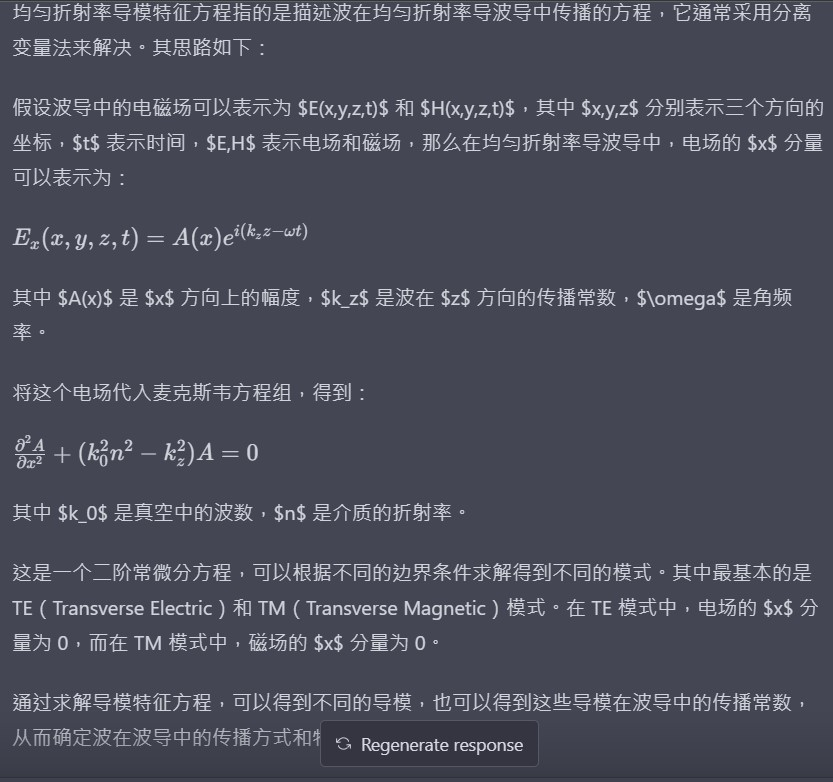
\includegraphics[width=8cm]{A.jpg}
    \caption{结果}
\end{figure}
\section{讨论渐变型光纤轨迹方程的思路?}
渐变型光纤可以用非线性微分方程组来描述,而光线在光纤中的传输可以由光线传输方程描述。因此,讨论渐变型光纤轨迹方程的思路可以分为以下几个步骤:

建立光线传输方程。光线传输方程描述了光线在渐变型光纤中的传输情况。根据光学原理和光线传输方程,可以求得光线的路径和传输特性。

求解非线性微分方程组。将渐变型光纤的折射率视为随机变量,则可以将非线性微分方程组转化为随机微分方程组,并应用随机微分方程的理论求解。

确定光纤轨迹方程。根据光线传输方程和非线性微分方程组的求解结果,可以确定渐变型光纤的轨迹方程和传输特性。

分析和讨论。根据光纤轨迹方程和传输特性,可以分析光线在光纤中的传输情况,包括光线传输的路径、速度、强度等参数,进而讨论渐变型光纤的应用和优化方向。


\section{费马原理及数学表示}

渐变型光纤可以用非线性微分方程组来描述,而光线在光纤中的传输可以由光线传输方程描述。因此,讨论渐变型光纤轨迹方程的思路可以分为以下几个步骤:

建立光线传输方程。光线传输方程描述了光线在渐变型光纤中的传输情况。根据光学原理和光线传输方程,可以求得光线的路径和传输特性。

求解非线性微分方程组。将渐变型光纤的折射率视为随机变量,则可以将非线性微分方程组转化为随机微分方程组,并应用随机微分方程的理论求解。

确定光纤轨迹方程。根据光线传输方程和非线性微分方程组的求解结果,可以确定渐变型光纤的轨迹方程和传输特性。

分析和讨论。根据光纤轨迹方程和传输特性,可以分析光线在光纤中的传输情况,包括光线传输的路径、速度、强度等参数,进而讨论渐变型光纤的应用和优化方向。

\section{费马原理及数学表示}
\begin{figure}[htbp][H]
    \centering
    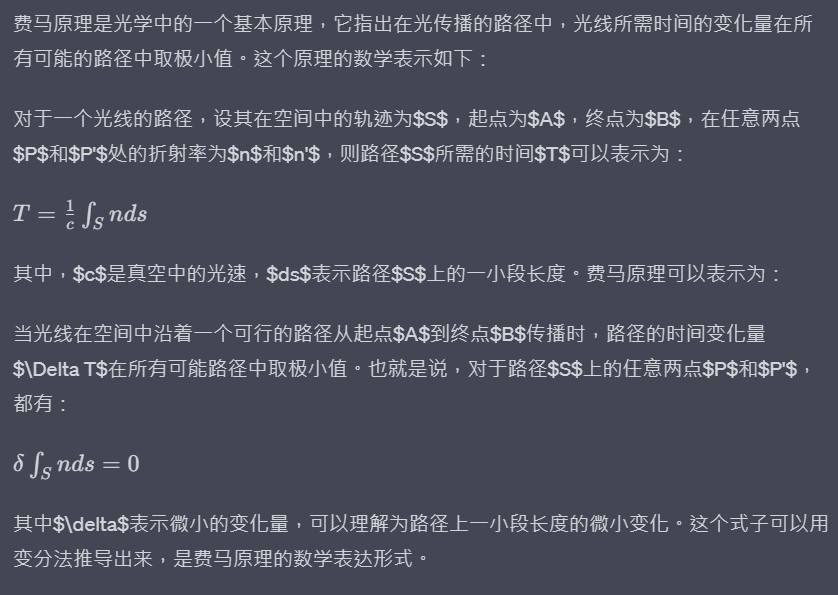
\includegraphics[width=8cm]{B.jpg}
    \caption{结果}
\end{figure}

\section{双曲正割型分布与平方律分布比较}
\begin{figure}[htbp][H]
    \centering
    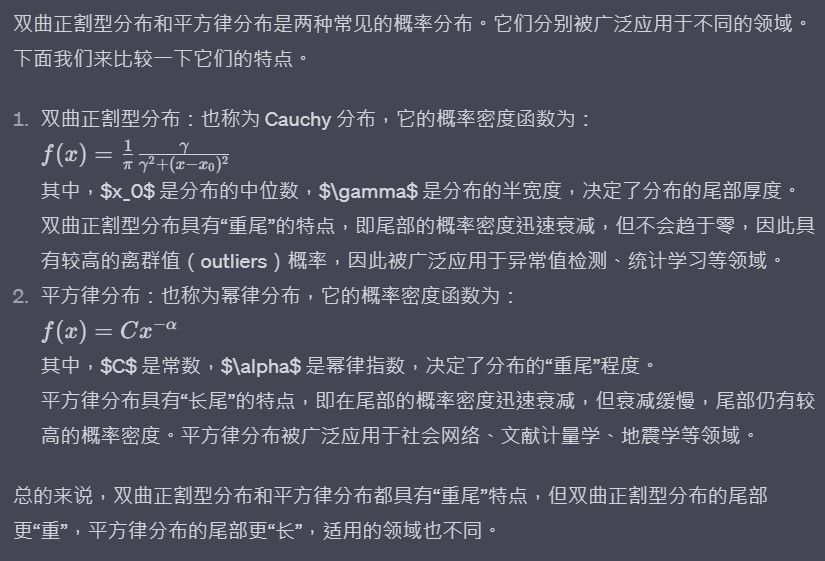
\includegraphics[width=8cm]{C.jpg}
    \caption{结果}
\end{figure}

\section{导波成立的条件与导波截止条件 }

导波是电磁波在导体中传输的一种形式,其在导体内的传输满足一定的条件。导波成立的条件是:
\\
存在导体:导波只能在有导体的介质中传播,因为电磁波必须与导体相互作用才能产生导波现象。
\\
电磁波频率低于临界频率:在导体中传输的电磁波频率不能高于导体的临界频率,临界频率是导体能够支持的最高频率,超过该频率,电磁波将不会传输。
\\
电磁波入射角度小于临界角:电磁波的入射角度也会影响导波的传输情况,当入射角度超过临界角时,电磁波将无法进入导体内部形成导波。
\\
导波截止条件是指当电磁波频率超过导体的临界频率时,导波将停止传输。这是由于高频电磁波无法被导体吸收,只能在导体表面上传播,而不能进入导体内部形成导波。因此,频率高于临界频率的电磁波无法在导体中传输,导波也将截止。

\section{模式的远离截止与接近截止 }
在波导中,模式是通过传播常数与介质中的特性阻抗相互作用而产生的。在一定范围内,模式可以传输信号,这个范围由截止条件来确定。

导波截止条件指的是,当工作频率低于截止频率时,导波结构不能传输电磁波,只能反射或吸收电磁波。在导波截止频率以下,介质中的损耗过大,使得波的传播过程中的损耗超过了增益,因此无法形成稳定的波。

接近截止条件指的是,当工作频率接近截止频率时,导波结构中的波的传播常数与空气中的传播常数之差变得非常小,此时,波的衰减与传播的距离呈指数关系,因此在接近截止频率时,波的衰减非常快。在实际设计中,需要避免频率接近截止频率,以免导致高衰减和不稳定的传输。


\section{分别说明Emny, Emnx意义  }
在电磁场理论中,Emny和Emnx分别表示电磁波的纵向和横向分量,其中Emny表示电磁波在y方向的纵向分量,Emnx表示电磁波在x方向的横向分量。

具体来说,对于一个电磁波,它的电场和磁场可以沿着不同的方向振动,这样就可以将电磁波分解为横波和纵波两部分。在横电磁波中,电场和磁场的振动方向垂直于波的传播方向;而在纵电磁波中,电场和磁场的振动方向与波的传播方向平行。

因此,Emny和Emnx分别描述了电磁波在垂直和平行于波的传播方向的振动。

\section{数值孔径的意义?有几种表示方式?}

数值孔径是光学系统的一个重要参数,它反映了光学系统的分辨能力和成像质量。它通常用于描述物镜或透镜的孔径大小和入射光束的角度范围。
数值孔径大的光学系统能够提供更高的分辨率和更清晰的图像,但相应的成本和复杂性也会增加。

数值孔径有几种不同的表示方式,其中最常见的是NA(Numerical Aperture,数值孔径)和f(f-number,F数)。
NA是指光学系统中物镜或透镜前的一组光线能够进入的最大角度,它与光线折射率和孔径直径有关。f是指物镜或透镜的焦距与孔径的比值,它可以用来表示光线通过光学系统的相对尺寸。两种表示方式在一定条件下可以互相转换。

除了NA和f之外,数值孔径还可以用波长和孔径直径的比值来表示,称为光学分辨率限制(Optical Resolution Limit,ORL)。
ORL可以用来表示光学系统的分辨率极限,即最小可分辨的空间尺度。


\section{什么是子午光线在光纤中的时延差?引起什么现象? }
子午光线是指光线沿着光纤的中心轴传播的路径。由于光纤的折射率是随径向变化的,所以不同径向位置的子午光线在传播过程中所经历的光程不同,导致子午光线的时延也不同。这种不同径向位置光线的时延差称为子午光线的时延色散。

子午光线的时延色散会导致信号的扩展,这是因为不同频率的光在光纤中的传播速度不同,造成信号在传输过程中的失真和色散。这种扩展和失真限制了光纤通信系统的带宽和传输距离。
因此,光纤通信系统中通常会采用一些措施来抑制子午光线的时延色散,例如使用带宽受限光源、使用色散补偿器等。
\section{简述高锟的主要贡献 }

成功研制出我国第一台氦氖激光器:1959年,高锟带领团队成功研制出我国第一台氦氖激光器,开创了我国激光研究的先河。

提出了“三步法”激光束整形方法:1963年,高锟提出了“三步法”激光束整形方法,使激光束在照射距离内不发散,成为国际上公认的激光束整形方法。

创立了中国的激光研究体系:1960年,高锟创办了中国第一个激光实验室,为我国激光研究奠定了基础。此后,他又先后创建了上海激光技术研究所和华东理工大学激光研究所,为中国激光事业培养了大批优秀的科技人才。


\section{为什么要研究折射率渐变型分布的光纤}
研究折射率渐变型分布的光纤是因为它们具有很多优良的特性,例如:
\\
渐变型折射率分布可以减小色散,提高带宽:光纤传输中的信号会因为折射率不同而导致不同的传播速度,进而引起色散。而采用折射率渐变型分布的光纤可以减小色散,提高带宽。
\\
渐变型折射率分布可以提高光纤的带宽利用率:折射率分布的变化可以改变光线的传输方向和模式,进而提高光纤的带宽利用率。
\\
渐变型折射率分布可以降低损耗:光纤的损耗与材料的吸收和散射有关,而折射率渐变型分布的光纤可以减少损耗,提高传输效率。
\\
渐变型折射率分布可以提高光纤的机械强度:光纤的折射率分布决定了光纤的弯曲半径,而折射率渐变型分布的光纤可以提高光纤的机械强度,降低光纤的损坏率。
\\
因此,研究折射率渐变型分布的光纤对于提高光纤传输的性能和可靠性具有重要意义。






\end{spacing}{}

\end{document}